\subsection{Struttura ed Esecuzione del Progetto}
All'interno della cartella principale del progetto è presente la cartella \texttt{source}, che contiene il codice sorgente del progetto, organizzato in 4 cartelle principali: \texttt{actors}, \texttt{crypto}, \texttt{models} e \texttt{simulation}.

\begin{figure}[H]
	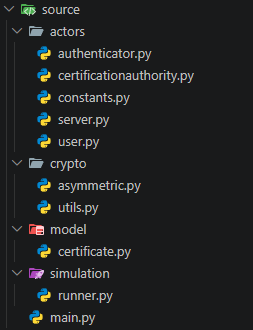
\includegraphics{./img/struttura_progetto.png}
	\centering
\end{figure}
In particolare:
\begin{itemize}
	\item \textbf{actors:} contiene le classi che rappresentano i vari attori del sistema (Utente, Authenticator, Server, CA).

	\item \textbf{crypto:} contiene le classi che implementano le primitive crittografiche utilizzate nel sistema (ad esempio, firme digitali, cifratura).

	\item \textbf{model:} contiene una classe wrapper per i certificati digitali, che semplifica la gestione dei certificati all'interno delle funzioni delle classi degli attori, nascondendo i dettagli di implementazione dei certificati digitali.\\
	In un'implementazione futura può essere ragionevole creare le classi wrapper per le strutture dati (come la VoterMap, il buffer dell'Authenticator e la lista dei nonce del server) e per i pacchetti scambiati tra gli attori, in modo da semplificare e rendere ancora più leggibile la comunicazione tra gli attori.

	\item \textbf{simulation:} contiene la funzione runner che simula l'intero processo di voto, dalla registrazione degli utenti alla pubblicazione dei risultati, per uno o più utenti, con la possibilità di visualizzare l'output dettagliato o sintetico del processo di voto. 
\end{itemize}

All'interno della cartella source del progetto è presente il file \texttt{main.py}, che permette di eseguire la simulazione. Quindi per avviare la simulazione dalla cartella principale del progetto, è possibile eseguire il comando:
\begin{lstlisting}
$ python ./source/main.py
\end{lstlisting}

\subsection{Simulazione e Output}
La simulazione crea un certo numero di utenti (specificato nel file \texttt{main.py}) e simula l'intero processo di voto per ciascun utente, dalla registrazione alla pubblicazione dei risultati. Solo per il primo utente viene mostrato l'output dettagliato del processo di voto, mentre per gli altri utenti viene mostrato solo l'output sintetico per non riempire il terminale.\\
Ciascuna fase definita dal protocollo viene mostrata in output con il dettaglio di tutte le operazioni eseguite da ciascun utente, evidenziando l'attore che sta eseguendo l'operazione col suo colore di riferimento ripreso dal diagramma di sequenza del protocollo.\\

Di seguito è riportato l'esempio di output dettagliato per la fase preliminare del sistema:
\begin{figure}[H]
	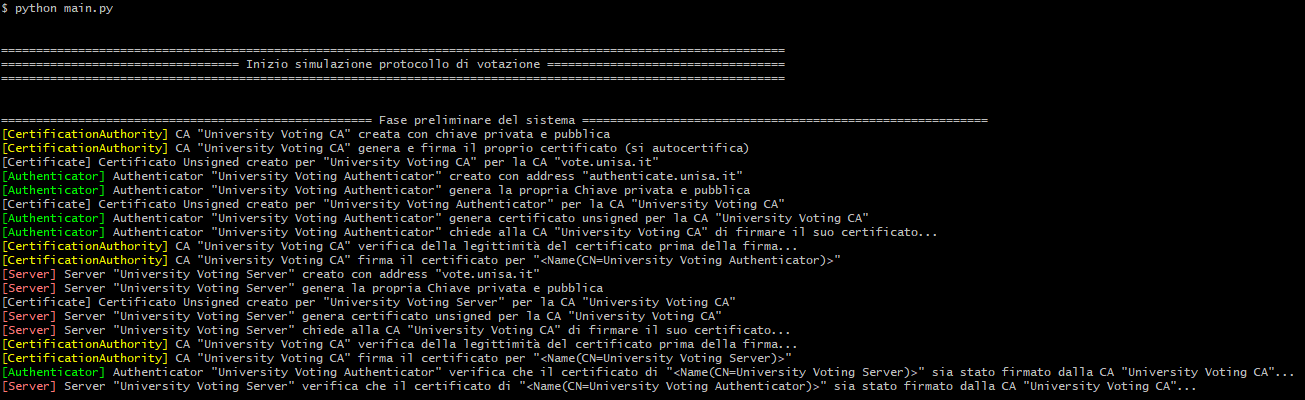
\includegraphics[width=1\textwidth]{./img/output_fase_preliminare.png}
	\centering
\end{figure}

Di seguito è riportato l'esempio di output della creazione di utenti:
\begin{figure}[H]
	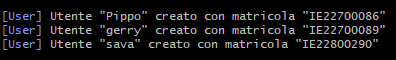
\includegraphics[width=.7\textwidth]{./img/output_user_creation.png}
	\centering
\end{figure}

Di seguito è riportato l'esempio di output dettagliato della simulazione per l'utente "Pippo" (il primo utente creato nella simulazione), differenziando le varie fasi del protocollo.\\
Fase certificato utente:
\begin{figure}[H]
	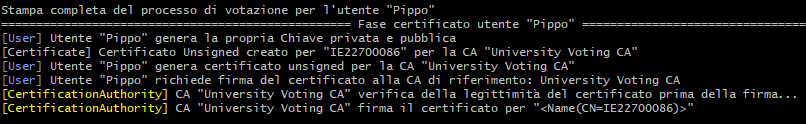
\includegraphics[width=1\textwidth]{./img/output_fase_certificato_utente.png}
	\centering
\end{figure}

Fase di handshake:
\begin{figure}[H]
	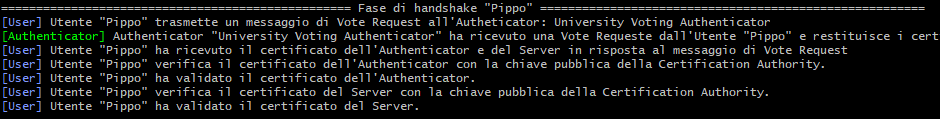
\includegraphics[width=1\textwidth]{./img/output_fase_handshake.png}
	\centering
\end{figure}

Fase trasmissione voto:
\begin{figure}[H]
	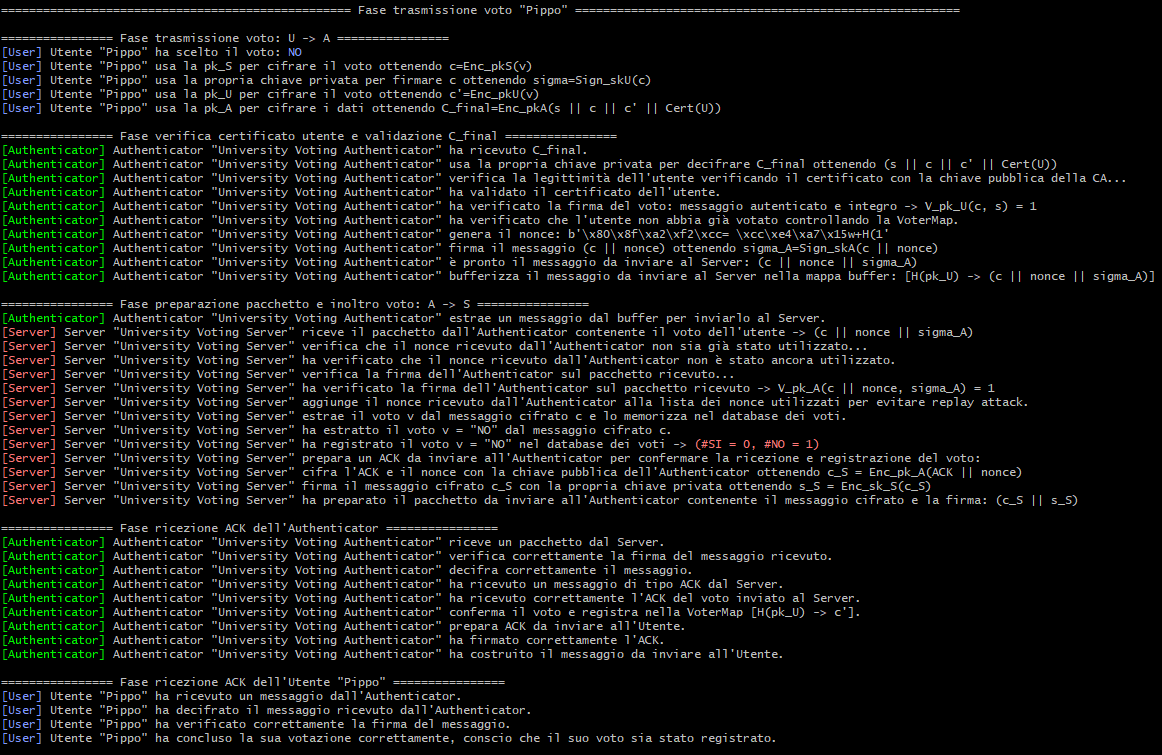
\includegraphics[width=1\textwidth]{./img/output_fase_trasmissione_voto.png}
	\centering
\end{figure}

Di seguito è riportato l'esempio di output della verifica individuale dei voti da parte dell'utente "Pippo":
\begin{figure}[H]
	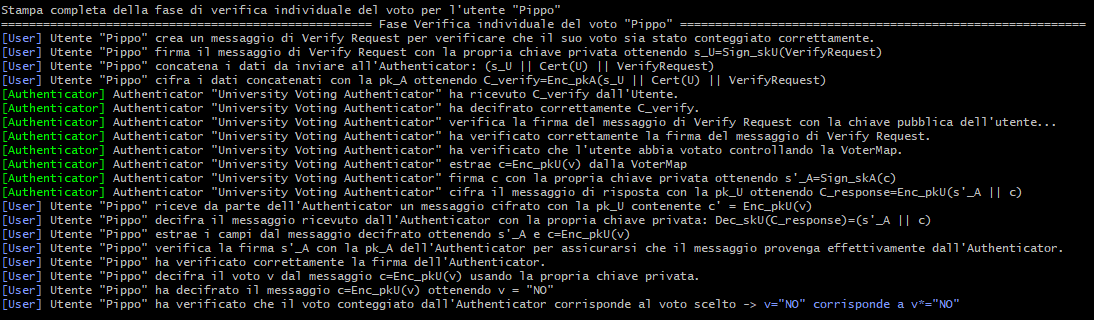
\includegraphics[width=1\textwidth]{./img/output_verifica_individuale.png}
	\centering
\end{figure}

Di seguito è riportato l'esempio di output della verifica universale dei voti da parte degli utenti:
\begin{figure}[H]
	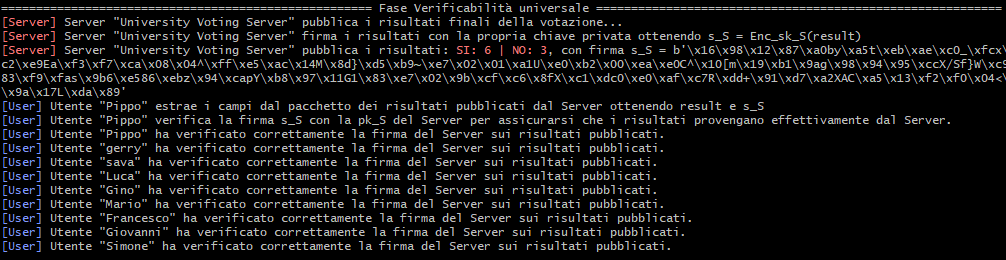
\includegraphics[width=1\textwidth]{./img/output_verifica_universale.png}
	\centering
\end{figure}

\subsection{Problema e miglioria futura}
Nella fase di trasmissione voto del protocollo stabilito, l'utente deve creare il cifrato $C_{final} = \text{Enc}_{pk_A}(\sigma \| c\| c'\| \text{Cert(U)})$ da inoltrare al server. Secondo il protocollo, il cifrato $C_{final}$ deve essere creato utilizzando l'algoritmo di cifratura asimmetrica RSA-OAEP, che prevede l'utilizzo di un padding randomico. Tuttavia si presenta l'impossibilità di cifrare interamente la concatenazione di $\sigma \| c\| c'\| \text{Cert(U)}$ con RSA-OAEP, in quanto la dimensione del messaggio da cifrare supera la dimensione massima consentita per la cifratura con RSA-OAEP (che dipende dalla dimensione della chiave pubblica utilizzata).\\
La scelta didattica per risolvere questo problema è stata quella di dividere il messaggio da cifrare in più parti, cifrando ciascuna parte separatamente con RSA-OAEP, ottenendo in questo modo un vettore di cifrati che rappresenta il cifrato finale $C_{final}$.\\
Ovviamente questa soluzione non è ottimale, in quanto se i singoli blocchi cifrati non sono crittograficamente legati tra loro, un attaccante sulla rete (attacco Man-in-the-Middle) potrebbe eliminare, duplicare o riordinare i blocchi cifrati alterando il messaggio finale senza invalidare le singole decifrature. Un altro problema è legato all'inefficienza computazionale, in quanto la cifratura asimmetrica è più lenta di quella simmetrica, quindi eseguire più cifrature asimmetriche per cifrare un messaggio di grandi dimensioni è inefficiente.\\
Una possibile soluzione a questo problema è quella di utilizzare una cifratura ibrida, in cui si genera una chiave di sessione R simmetrica casuale (ad esempio, utilizzando AES) per cifrare l'intero messaggio $(\sigma \| c\| c'\| \text{Cert(U)})$ con un algoritmo di cifratura simmetrica, ottenendo in questo modo il cifrato $C_{final}$. Per adottare questa soluzione, è necessario modificare il protocollo stabilito, aggiungendo un passaggio in cui l'utente genera la chiave di sessione R simmetrica casuale e la cifra con la chiave pubblica dell'Authenticator, utilizzando RSA-OAEP, ottenendo in questo modo un cifrato $C_R = \text{Enc}_{pk_A}(R)$. Successivamente, l'utente cifra l'intero messaggio $(\sigma \| c\| c'\| \text{Cert(U)})$ con la chiave di sessione R utilizzando un algoritmo di cifratura simmetrica (ad esempio AES), ottenendo in questo modo il cifrato $C_{final} = \text{Enc}_R(\sigma \| c\| c'\| \text{Cert(U)})$. Infine, l'utente invia all'Authenticator sia il cifrato $C_R$ che il cifrato $C_{final}$, e il server decifra prima $C_R$ con la propria chiave privata per ottenere la chiave di sessione R, e successivamente decifra $C_{final}$ con la chiave di sessione R per ottenere il messaggio originale $(\sigma \| c\| c'\| \text{Cert(U)})$.\\
Questa soluzione è più sicura, in quanto la chiave di sessione R è crittografata con la chiave pubblica dell'Authenticator, quindi solo l'Authenticator può decifrarla.